\documentclass[english]{article}

\bibliographystyle{unsrt}

% Section
\newcommand{\secref}[1]{Subsection~\ref{sec.#1}}
\newcommand{\seclabel}[1]{\label{sec.#1}}

% Appendix
\newcommand{\appref}[1]{Appendix~\ref{app.#1}}
\newcommand{\applabel}[1]{\label{app.#1}}

% Table
\newcommand{\tabnum}[1]{\ref{tab.#1}}
\newcommand{\tabref}[1]{Table~\tabnum{#1}}
\newcommand{\tablabel}[1]{\label{tab.#1}}

% Equation
\newcommand{\eqnref}[1]{Equation~\ref{Equations.#1}}
\newcommand{\eqnlabel}[1]{\label{Equations.#1}}

% Figure
\newcommand{\figref}[1]{Figure~\ref{Figures.#1}}
\newcommand{\figlabel}[1]{\label{Figures.#1}}

\newcommand{\easyfig}[4]{
\begin{figure}
\includegraphics[#2]{#1}
\caption{ \figlabel{#3} #4}
\end{figure}}

\newcommand{\dotfig}[4]{
\begin{figure}
\input{#1.tex}
\includegraphics[#2]{#1.ps}
\caption{ \figlabel{#3} #4}
\end{figure}}

\newcommand{\pngfig}[2]{\easyfig{#1.png}{}{#1}{#2}}
\newcommand{\pdffig}[2]{\easyfig{#1-fig.pdf}{}{#1}{#2}}

\newcommand{\widepngfig}[2]{\easyfig{#1.png}{width=\textwidth}{#1}{#2}}
\newcommand{\tallpngfig}[2]{\easyfig{#1.png}{height=.8\textheight}{#1}{#2}}
\newcommand{\widepdffig}[2]{\easyfig{#1-fig.pdf}{width=\textwidth}{#1}{#2}}
\newcommand{\tallpdffig}[2]{\easyfig{#1-fig.pdf}{height=.8\textheight}{#1}{#2}}

\newcommand{\sidewayspngfig}[2]{
\begin{sidewaysfigure}
\includegraphics[width=\textwidth]{#1.png}
\caption{\figlabel{#1} #2}
\end{sidewaysfigure}
}

% ToDo
\newcommand{\needfig}[1]{{\bf Need figure: } #1 }
\newcommand{\needfigref}[1]{Figure~??? [#1] }

\newcommand{\needcite}[1]{[CITE #1]}
\newcommand{\todo}[1]{[TODO: #1]}

% Packages

\usepackage[boxed,noend]{algorithm2e}
\usepackage{graphicx}
\usepackage{psfrag}
\usepackage{url}
\usepackage{amsmath}
\usepackage{amssymb}
\usepackage{color} 
\usepackage{ifthen}
\usepackage{rotating}
\newcommand{\hl}[1]{#1}

\newcommand\semiring{K}
\newcommand\srset{\mathbb{K}}
\newcommand\srplus{\oplus}
\newcommand\srtimes{\otimes}
\newcommand\srplusid{\underline{0}}
\newcommand\srtimesid{\underline{1}}
\newcommand\srsum{\bigoplus}
\newcommand\srprod{\bigotimes}

\newcommand\inalph{\Sigma}
\newcommand\outalph{\Omega}
\newcommand\states{Q}
\newcommand\transitions{E}
\newcommand\initstate{i}
\newcommand\finalstate{f}
\newcommand\emptystring{\epsilon}
\newcommand\maybe[1]{#1 \cup \{ \emptystring \}}

\newcommand\state{q}
\newcommand\trans{t}
\newcommand\src{p}
\newcommand\dest{q}
\newcommand\lab{\ell}
\newcommand\inlab{\lab_i}
\newcommand\outlab{\lab_o}
\newcommand\weight{\mathbb{W}}

\newcommand\somealph{\Gamma}
\newcommand\someseq{\gamma}
\newcommand\midlab{\lab_m}

\newcommand\transcomp{\circ}
\newcommand\transconcat{+}

\newcommand\inseq{\sigma}
\newcommand\outseq{\omega}

\newcommand\kleene[1]{{#1}^{\ast}}
\newcommand\inseqs{\kleene{\inalph}}
\newcommand\outseqs{\kleene{\outalph}}
\newcommand\someseqs{\kleene{\somealph}}

\newcommand\tfunc[1]{\mathbb{#1}}

\newcommand\bigo{{\cal O}}

\newcommand\seqof[1]{\bar{#1}}
\newcommand\sympast{v}
\newcommand\symnext{w}
\newcommand\seqpast{\seqof{\sympast}}
\newcommand\seqnext{\seqof{\symnext}}

\newcommand\nucalph{\somealph_{\mbox{\tiny DNA}}}
\newcommand\sym{x}
\newcommand\comp[1]{\tilde{#1}}
\newcommand\revcomp[1]{\comp{#1}}
\newcommand\ntrans[1]{\hat{#1}}
\newcommand\seqlen[1]{|#1|}
\newcommand\otherseq{\lambda}

\newcommand\kmerlen{{\cal K}}
\newcommand\invreplen{L_{\mbox{\tiny invrep}}}

\newcommand\graph{{\cal G}}
\newcommand\vertices{{\cal V}}
\newcommand\edges{{\cal E}}

\newcommand\debruijngraph{\graph_b}
\newcommand\debruijnvertices{\vertices_b}
\newcommand\debruijnedges{\edges_b}

\newcommand\norepgraph{\graph_r}
\newcommand\norepvertices{\vertices_r}
\newcommand\norepedges{\edges_r}

\newcommand\controlgraph{\graph_c}
\newcommand\controlbridges[1]{\vertices_c(#1)}

\newcommand\prequels{{\cal S}}
\newcommand\stepsto{{\cal L}}

\newcommand\ncontrols{N_c}
\newcommand\controlset{{\cal M}}
\newcommand\controlword{M}

\newcommand\initword{\controlword_i}
\newcommand\finalword{\controlword_f}

\newcommand\initvertex[1]{u^{(#1)}_i}
\newcommand\finalvertex[1]{v^{(#1)}_f}

\newcommand\controlmachine{T_c}

\newcommand\bit[1]{#1_2}
\newcommand\trit[1]{#1_3}
\newcommand\quat[1]{#1_4}
\newcommand\controlsym[1]{{#1}_M}
\newcommand\flushsym{F}

\newcommand\figtrans[2]{T_{\ref{Figures.#1}#2}}
\newcommand\solefigtrans[1]{T_{\ref{Figures.#1}}}

\newcommand\transsingle[2]{T_{#1 \to #2}}
\newcommand\transid[1]{\transsingle{#1}{#1}}
\newcommand\transerase[1]{\transsingle{#1}{\epsilon}}

\newcommand\rbit[1]{#1_{2R}}

\newcommand\hammingthreeone{\figtrans{HammingTransducer}{a}}
\newcommand\hammingsevenfour{\figtrans{HammingTransducer}{b}}

\newcommand\transbintoquat{\figtrans{NaiveDNATransducer}{a}}
\newcommand\transquattodna{\figtrans{NaiveDNATransducer}{b}}
\newcommand\transbintodna{\figtrans{NaiveDNATransducer}{c}}

\newcommand\transdivthree{\figtrans{DivisionByThree}{a}}
\newcommand\transternzeroid{\figtrans{DivisionByThree}{b}}
\newcommand\transternsymid{\figtrans{DivisionByThree}{c}}
\newcommand\transternseqid{\figtrans{DivisionByThree}{d}}
\newcommand\transerasezerobits{\figtrans{DivisionByThree}{e}}
\newcommand\transechodivthree{\figtrans{DivisionByThree}{f}}

\newcommand\transmixed{\figtrans{Converter}{a}}
\newcommand\transflush{\figtrans{Converter}{b}}

\newcommand\transechodivtwo{\figtrans{EvenDivision}{a}}
\newcommand\transechodivfour{\figtrans{EvenDivision}{b}}
\newcommand\transechodivmixed{T_{2 \to 234}}

\newcommand\transpartial{\figtrans{PartialObservation}{c}}

\newcommand\nuc[1]{\mbox{#1}}
\newcommand\nuca{\nuc{A}}
\newcommand\nucc{\nuc{C}}
\newcommand\nucg{\nuc{G}}
\newcommand\nuct{\nuc{T}}

\newcommand\contextlen{L}
\newcommand\seqsyms[2]{\sym_{#1} \ldots \sym_{#2}}
\newcommand\seqpastsyms[2]{\sympast_{#1} \ldots \sympast_{#2}}
\newcommand\seqnextsyms[2]{\symnext_{#1} \ldots \symnext_{#2}}
\newcommand\outsym{y}

\newcommand\param[1]{\mathbb{P}_{#1}}

\newcommand\pnogap{\param{n}}
\newcommand\pdelopen{\param{d}}
\newcommand\ptandup{\param{t}}
\newcommand\pfwddup{\param{f}}
\newcommand\prevdup{\param{r}}

\newcommand\pdelext{\param{x}}
\newcommand\pdelend{\param{e}}

\newcommand\pmatch{\param{m}}
\newcommand\ptransition{\param{i}}
\newcommand\ptransversion{\param{v}}

\newcommand\submat{\param{s}}
\newcommand\lendist{\param{l}}

\newcommand\psub{\submat(\sym,\outsym)}
\newcommand\psubnext[1]{\submat(\symnext_{#1},\outsym)}
\newcommand\psubpast[1]{\submat(\sympast_{#1},\outsym)}
\newcommand\psubcomppast[1]{\submat(\sympast_{#1},\comp{\outsym})}
\newcommand\psubcompnext[1]{\submat(\symnext_{#1},\comp{\outsym})}

\newcommand\plen[1]{\lendist(#1)}

\newcommand\pcont{\pnogap^\ast}

\newcommand\block{\alpha}
\newcommand\srcblock{\block}
\newcommand\destblock{\beta}

\newcommand\blockstate[2]{{#1}_{#2}}
\newcommand\lenstate[3]{\blockstate{#1}{#2}^{(#3)}}

\newcommand\symstate[1]{\blockstate{S}{#1}}
\newcommand\delstate[1]{\blockstate{D}{#1}}
\newcommand\tanstate[2]{\lenstate{T}{#1}{#2}}
\newcommand\fwdstate[2]{\lenstate{F}{#1}{#2}}
\newcommand\revstate[2]{\lenstate{R}{#1}{#2}}

\begin{document}

\newcommand\authorstring{
Ian Holmes$^{1,\ast}$ \\
\textbf{1} Department of Bioengineering, University of California, Berkeley, CA, USA \\
$\ast$ E-mail: ihh@berkeley.edu
}

\newcommand\titlestring{Transducer codes for DNA}
\newcommand\shorttitlestring{Transducer codes for DNA}
\markboth{\shorttitlestring}{\shorttitlestring}
\begin{flushleft}
{\Large \textbf{\titlestring} } \\
\authorstring
\end{flushleft}
%\section{Abstract}
%\paragraph{Keywords:}
%\tableofcontents

\section{Introduction}

DNA storage \cite{ChurchEtAl2012,GoldmanEtAl2013}.
Codes \cite{YazdiEtAl2015}


\cite{GoldmanEtAl2013} use a trinary (radix-3) code that avoids repeated nucleotides in the synthesized DNA
Their argument is that this protects against most common class of errors in DNA resequencing which occur at homopolymer runs
However, this is just one point on a spectrum of possibilities
Different applications might require different codes
e.g. if synthesis is cheap and sequencing is error-prone, then use error-tolerant codes that may add overhead, but want to keep overhead as low as possible
Or if archiving data for retrieval in distant future, given current market where synthesis remains expensive and sequencing is becoming ever cheaper and more accurate, might be better to pack as much information into the DNA as possible --- but there may still be a need to interleave metadata, escape sequences, biological motifs, or other ``reserved words'' into the DNA sequence

Here we present a modular, rational strategy for designing codes that meet such flexible needs
including error-avoidance, error-correction, and demarcated metadata

Our strategy represents different stages of the encoding and decoding process
modularly as state machines.
This eases the process of designing the codec,
allows easy incorporation of error-correcting codes
(Hamming codes, convolutional ``turbo codes'')
and allows us to introduce a statistically-parameterized model of errors
in DNA sequencing and replication,
and use Viterbi algorithm for decoding

For representing these modular operations on state machines,
the most appropriate technology is the finite-state transducer \cite{MohriPereiraRiley2000,WikipediaTransducers}
In bioinformatics:
protein classification \cite{EskinEtAl2000},
phylogenetics \cite{PatenEtAl2008,WestessonEtAlArxiv2012,WestessonEtAl2012},
cancer informatics \cite{SchwarzEtAl2014}

Desired features of the code:
repeat avoidance,
reserved words (e.g. barcoding,
identification of start and end of files,
insertion of other filesystem metadata facilitating random access or scaffolded reassembly,
escape sequences,
insertion of biologically relevant motifs e.g. restriction enzyme sites)

De Bruijn graphs \cite{DeBruijn1946,PevznerEtAl2001,ZerbinoBirney2008,IqbalEtAl2012}
and relationship to automata with limited context e.g. order-$N$ Markov models


\section{Methods}

\subsection{Weighted finite-state transducers}

Following \cite{MohriPereiraRiley2000}:
Assume a general semiring
$\semiring=(\srset,\srplus,\srtimes,\srplusid,\srtimesid)$
which for our purposes is typically the probability semiring
$(\Re,+,\times,0,1)$
or the tropical semiring
$(\Re_{+} \cup {\infty},\min,+,\infty,0)$.

A weighted finite-state transducer is defined as a tuple
$T = (\inalph,\outalph,\states,\transitions,\initstate,\finalstate)$
consisting of an input alphabet $\inalph$,
an output alphabet $\outalph$ (both alphabets being finite sets),
a finite set of states $\states$,
a finite set of transitions
$\transitions \subseteq \states \times (\maybe{\inalph}) \times (\maybe{\outalph}) \times \srset \times \states$,
an initial state $\initstate \in \states$
and a final state $\finalstate \in \states$.

The transducer $T$ can be thought of as an edge-labelled directed graph
where each state is a vertex
and each transition
$\trans = (\src[\trans],\inlab[\trans],\outlab[\trans],\weight[\trans],\dest[\trans]) \in \transitions$
is an edge from state $\src[\trans]$ to state $\dest[\trans]$
with input label $\inlab[\trans]$,
output label $\outlab[\trans]$
and weight $\weight[\trans]$.
For the figures in this paper,
we adopt the convention that transition labels are annotated as $\inlab{\tt /}\outlab$
(the transition weights for the transducers in the figures are all equal to 1, and are not shown).
\figref{HammingTransducer} shows a transducer that implements the Hamming(3,1) error-correcting code,
\figref{NaiveDNATransducer} shows a transducer that converts a binary string into DNA,
and
\figref{DivisionByThree} shows a transducer that implements division by 3.

A path in $T$ is a series of transitions that form a path in this graph.
The input sequence and output sequence for a path are the concatenation of (respectively)
the input and output labels of the transitions in the path.
The path weight is the $\srtimes$-product of the transition weights.
A successful path is one that starts in $\initstate$ and ends in $\finalstate$.
The transduction weight for a given input sequence $\inseq \in \inseqs$
and output sequence $\outseq \in \outseqs$
is the $\srplus$-sum of all successful paths
having $\inseq$ as the input sequence
and $\outseq$ as the output sequence.
Thus $T$ provides a mapping
$\tfunc{T}:(\kleene{\inalph} \times \kleene{\outalph}) \to \srset$
from sequence-pairs to weights.
We call this mapping $\tfunc{T}$ the transducer function.
For a given pair of sequences $(\inseq,\outseq)$
and a semiring wherein $\srplus$ and $\srtimes$ are amortized-constant resource operations,
it can be evaluated in time $\bigo(|\inseq| \cdot |\outseq| \cdot |\transitions|)$
and memory $\bigo(|\inseq| \cdot |\outseq| \cdot |\states|)$
by dynamic programming,
analogously to the Forward algorithm in the probabilistic semiring
or the Viterbi algorithm in the tropical semiring
\cite{Durbin98}.

A state $\state \in \states$ has past input context $\inseqpast$ if every path from $\initstate$ to $\state$ has an input sequence with suffix $\inseqpast$,
and future input context $\inseqnext$ if every path from $\state$ to $\finalstate$ has an input sequence with prefix $\inseqnext$.
The past output context and future output context of a state are defined similarly.


\subsection{Transducer composition}

Given transducers
 $R = (\inalph, \somealph, \states_R, \transitions_R, \initstate_R, \finalstate_R)$ and
 $S = (\somealph, \outalph, \states_S, \transitions_S, \initstate_S, \finalstate_S)$
where $R$'s output alphabet is the same as $S$'s input alphabet,
we can readily find a composite transducer
 $T = R \transcomp S = (\inalph, \outalph, \states_T, \transitions_T, \initstate_T, \finalstate_T)$
such that, if $\tfunc{R}$, $\tfunc{S}$ and $\tfunc{T}$ are the corresponding transducer functions,
then
\[
\forall \inseq \in \inseqs, \outseq \in \outseqs:
\quad
\tfunc{T}(\inseq,\outseq) = \srsum_{\someseq \in \someseqs} \tfunc{R}(\inseq,\someseq) \tfunc{R}(\someseq,\outseq)
\]
that is, $T$ models the feeding of $R$'s output into $S$'s input
(and this intermediate sequence is then summed out---i.e. marginalized, if we are in the probabilistic semiring).

Loosely speaking, we can construct $T$ using the following recipe:
\begin{itemize}
\item Each $T$-state corresponds to a pair of $R$- and $S$-states,
so $\state_T = (\state_R, \state_S)$
and $\states_T \subseteq \states_R \times \states_S$.
\item The initial $T$-state $\initstate_T=(\initstate_R,\initstate_S)$ pairs the initial states of $R$ and $S$.
\item The final $T$-state $\finalstate_T=(\finalstate_R,\finalstate_S)$ pairs the final states of $R$ and $S$.
\item $T$-transitions
$\trans_T = ((\src_R,\src_S),\inlab,\outlab,\weight_T,(\dest_R,\dest_S))$
represent (summaries of sets of) synchronized pairs of $R$-transitions
$\trans_R = (\src_R,\inlab,\midlab,\weight_R,\dest_R)$
and $S$-transitions
$\trans_S = (\src_S,\midlab,\outlab,\weight_S,\dest_S)$
which share the same intermediate label $\midlab$.
The composite transition weight $\weight_T$ is the product $\weight_R \srtimes \weight_S$,
or the sum over such products if there are multiple transition-pairs $(\trans_R,\trans_S)$
consistent with a given $\trans_T$
(which, in the probabilistic semiring, is equivalent to marginalizing out $\midlab$).
\item Some additional manipulation is required to synchronize
transitions involving empty input labels (``insertions''),
empty output labels (``deletions''),
or both (``null transitions'').
For example, we can require that $S$-transitions accepting incoming symbols
all originate from ``ready'' states which have no outgoing insertions.
(If $S$ does not comply with this stipulation then we can easily derive a transducer
with the same transducer function $\tfunc{S}$ that does comply.)
\end{itemize}

This algorithm can be made precise enough to automate;
more detailed workings are given elsewhere \cite{PereiraRiley1996,MohriPereiraRiley2000,Holmes2003,Holmes2007,WestessonEtAlArxiv2012,WestessonEtAl2012}.
A simple example of transducer composition is shown in \figref{NaiveDNATransducer}.

\subsection{Transducer union and Kleene closure}

% WRITE ME
\figref{DivisionByThree}

\subsection{Transducer concatenation}

Anther operation on transducers that is useful in constructing DNA codes
is concatenation.
Suppose
 $A = (\inalph, \outalph, \states_A, \transitions_A, \initstate_A, \finalstate_A)$ and
 $B = (\inalph, \outalph, \states_B, \transitions_B, \initstate_B, \finalstate_B)$
are transducers with the same input and output alphabets and disjoint state spaces.
The concatenated transducer $T = A \transconcat B$ can be constructed by
taking the union of the state spaces and adding a null ($\epsilon/\epsilon$) unit weight transition
from $\finalstate_A$ to $\initstate_B$.
This models feeding the part of a sequence through $A$ and then feeding the second part through $B$.
Some simple examples of concatenation are shown in \figref{DivisionByThree}.

\subsection{De Bruijn graphs}

Denote by $\somealph^\kmerlen$
the set of all possible $\kmerlen$-symbol strings
$\sym_1 \sym_2 \ldots \sym_\kmerlen$ over some alphabet $\somealph$.

The $\kmerlen$-dimensional De Bruijn graph over $\somealph$
has vertex set $\somealph^\kmerlen$
and a directed edge $u \to v$ between any two vertices
$u=\sym_1 \sym_2 \ldots \sym_\kmerlen$ and $v=\sym_2 \ldots \sym_\kmerlen \sym_{\kmerlen+1}$
that overlap by $\kmerlen-1$ symbols; this edge is labeled with symbol $\sym_{\kmerlen+1}$ (the last symbol of $v$).
Thus, each vertex has $|\somealph|$ incoming and $|\somealph|$ outgoing edges \cite{DeBruijn1946,PevznerEtAl2001}.
Denote this graph by $\debruijngraph(\somealph^\kmerlen) = (\somealph^\kmerlen,\debruijnedges(\somealph^\kmerlen))$.

\subsection{DNA alphabets and repeats}

Let $\nucalph = \{ \mbox{A}, \mbox{C}, \mbox{G}, \mbox{T} \} $ be the nucleotide alphabet.
Let $\comp{x}$ denote the complement of a nucleotide symbol $x$,
and $\revcomp{\someseq}$ the reverse complement of a nucleotide sequence $\someseq$.
Let $\ntrans{x}$ denote the nucleotide related to $x$ by a transition substitution
(so $\ntrans{\nuca} = \nucg$, $\ntrans{\nucc}=\nuct$, etc.).

A direct tandem repeat of length $k$ is a nucleotide sequence followed by an exact copy of itself, $\someseq \someseq$, where the length of each copy is $\seqlen{\someseq}=k$
(note this includes repeated single nucleotides when $k=1$).
Similarly, a direct inverted repeat of length $k$ is a $k$-nucleotide sequence followed by its reverse complement, $\someseq \revcomp{\someseq}$.
A local inverted repeat of length $k$ and separation $l$ is a $k$-nucleotide sequence, followed an $l$-nucleotide sequence, followed by the reverse complement
of the first sequence; that is, $\someseq \otherseq \revcomp{\someseq}$, where $\seqlen{\someseq}=k$ and $\seqlen{\otherseq}=l$.

\subsection{A transducer for encoding signals as DNA without short repeats or reserved words}
\seclabel{DeBruijnTransducer}

Start with $\debruijngraph(\nucalph^\kmerlen)$, the $\kmerlen$-dimensional De Bruijn graph over $\nucalph$.
Delete all nodes corresponding to sequences that contain substrings which are
direct tandem repeats of any length,
direct inverted repeats of length $\geq 2$,
or local inverted repeats of length $\geq \invreplen$ and separation $\geq 2$.
Denote the resulting graph by $\norepgraph = (\norepvertices,\norepedges)$.

Let $A \subset \norepvertices$ be a set of vertices to avoid,
let $D \in A$ be a target vertex,
and denote by $\prequels(D,A,N) \subset \norepvertices$
the set of all vertices
from which there exists a length-$N$ path to $D$
that does not pass through any of the vertices in $A$
(although the path is allowed to originate from one of those vertices).
Define $\stepsto(D,A)$ to be the smallest value of $N$ for which $\prequels(D,A,N) = \norepvertices$,
if such a value of $N$ exists; otherwise, let $\stepsto(D,A)$ be $\infty$.
We can find $\prequels(D,A,N)$ from $\prequels(D,A,N-1)$ by recursive backtracking,
and so determine in $k$ steps whether $\stepsto(D,A) \leq k$.

We now allocate $\ncontrols$ ``control words'': $\kmerlen$-mers are reserved for marking metadata boundaries,
including the starts and ends of messages.
In the transducer, these will be unreachable except by specially constructed paths of uniform length.
Specifically, we seek an indexed set of vertices
$\controlset = \{ \controlword_1, \controlword_2 \ldots \controlword_{\ncontrols} \}$
such that $\stepsto(\controlword_n,\controlset) \leq k$ for all $n$
and for some pre-specified value of $k$.
Our implementation finds this list $\controlset$ by brute-force recursive search
(using $k = 2\kmerlen$)
and further attempts to maximize the shortest Hamming distance between any two control words in $\controlset$.
Note that there is a ceiling to the number of control words that may be found
for any given value of $\kmerlen$ (and $\invreplen$),
though this ceiling grows rather rapidly with $\kmerlen$.
In practice we only need a few control words for most purposes.

Having designated some $\kmerlen$-mers as control words via analysis of $\norepgraph$,
we now construct a new graph $\controlgraph$
in which the control words are unreachable from the other words
except by paths that we construct.
Starting with graph $\norepgraph$, delete all incoming transitions to control words $\controlword_n \in \controlset$,
rendering them unreachable,
and prune the graph of any other nodes that become unreachable as a result.
Next, for every control word $\controlword_n \in \controlset$
and every path length $1 \leq k < \stepsto(\controlword_n,\controlset)$,
we create a new vertex set $\controlbridges{n,k}$
with a one-to-one correspondence to $\prequels(\controlword_n,\controlset,k)$.
We connect the newly-added vertices such that there is an edge from
$u \in \controlbridges{n,k}$ to $v \in \controlbridges{n,k-1}$
for every corresponding edge $(u',v') \in \norepedges$ between
$u' \in \prequels(\controlword_n,\controlset,k)$
and
$v' \in \prequels(\controlword_n,\controlset,k-1)$.
We also add edges from
$u \in \norepvertices$ to $v \in \controlbridges{n,\stepsto(\controlword_n,\controlset)}$
for the first steps in the paths to control words,
as well as edges from
$u \in \controlbridges{n,1}$ to $\controlword$
for the final steps.
In each case the newly-added edge is copied from a corresponding edge in $\norepedges$
and inherits the same edge label.

It can be useful to force the transducer to start with a particular control word $\initword$
and finish with another (or the same) control word $\finalword$.
To guarantee this we can add a chain of initial vertices and edges leading from source vertex to the initial control word,
$\initvertex{0} \to \initvertex{1} \to \initvertex{2} \to \ldots \to \initvertex{\kmerlen-1} \to \initword$,
with each transition labeled with consecutive symbols from the initial control word.
We also need to add a transition from the final control word to the final state.
(If the start and end control words are the same, then this vertex should be duplicated to prevent cycles.)

We have now constructed the graph $\controlgraph$ from which our transducer $\controlmachine$
is derived via the following recipe:
\begin{itemize}
\item Every vertex in $\controlgraph$ is a state in $\controlmachine$.
The initial and final vertices of $\controlgraph$ are the initial and final states of $\controlmachine$.
\item Every edge in $\controlgraph$ is a unit-weight transition in $\controlmachine$.
The output label of the transition is the label of the edge.
\item The input label of each transition is determined as follows:
\begin{itemize}
\item For states in $\norepvertices$ with two outgoing transitions to other states in $\norepvertices$, those transitions are input-labeled with the binary digits (bits) $\bit{0}$ and $\bit{1}$.
\item For states in $\norepvertices$ with three outgoing transitions to other states in $\norepvertices$, those transitions are input-labeled with the trinary digits (trits) $\trit{0}$, $\trit{1}$ and $\trit{2}$.
\item For states in $\norepvertices$ with four outgoing transitions to other states in $\norepvertices$, those transitions are input-labeled with the quaternary digits (quats) $\quat{0}$, $\quat{1}$, $\quat{2}$ and $\quat{3}$.
\item Transitions from states in $\norepvertices$ to states in $\controlbridges{n,\stepsto(\controlword_n,\controlset)}$,
which begin a path to the $n$'th control word $\controlword_n$,
are input-labeled with the special control digit $\controlsym{n}$.
\item All other transitions have input label $\emptystring$.
\end{itemize}
\end{itemize}

Thus, the input alphabet of $\controlmachine$
is $\{ \bit{0}, \bit{1},
       \trit{0}, \trit{1}, \trit{2},
       \quat{0}, \quat{1}, \quat{2}, \quat{3},
       \controlsym{1} \ldots \controlsym{\ncontrols} \}$.

\figref{DNAStore} illustrates some of the code transducers that are generated by this procedure for the simplest case $\kmerlen=2$.
       
\subsection{A transducer with past and future context}

By virtue of being derived from the De Bruijn graph, most of the states in the transducer of \secref{DeBruijnTransducer}
have $\kmerlen$ nucleotides of past output context.
We can transform this transducer into an equivalent one wherein most of the states have
$\kmerlen/2$ nucleotides of past output context
and $\kmerlen/2$ nucleotides of future output context.

This can be a convenient way to think about context, for the purpose of modeling errors in DNA replication and sequencing.
Common decoding and replication errors include local tandem and inverted duplications, as well as context-dependent substitutions.
These can occur on either strand of and therefore (depending on the representation) may be best represented as depending
on future context as well as past context.

The transformation requires that the output sequence of all successful paths through the transducer
begin with a particular $\kmerlen$-mer and end with a particular $\kmerlen$-mer,
which can be ensured using the method described in \secref{DeBruijnTransducer}.

Let $\someseq = \inseqpast(\state)$ be the past output context for a given state $\state$.
All of the transitions $\trans$ into $\state$ have the same input label $\inlab[\trans] \equiv \inlab[\state]$,
which corresponds to the most recent nucleotide of output context for that state,
i.e. the $\kmerlen$'th symbol of $\someseq$.
If, instead, we set $\inlab[\trans]$ to be the $(\kmerlen/2)$'th symbol of $\someseq$
for all transitions into $\state$, then we have effectively delayed all output by $\kmerlen/2$ symbols.
We can now predict the next $\kmerlen/2$ symbols in the output sequence for the path from a state,
so we have traded $\kmerlen/2$ of past output context for $\kmerlen/2$ of future output context.

We need to add $\kmerlen/2$ extra padding states after (what was originally) the final state,
with a chain of transitions that flushes out the final $\kmerlen/2$ delayed output symbols.
Conversely, the first $\kmerlen/2$ transitions from the initial state
(into states with $\kmerlen/2$ or fewer nucleotides of output context)
will, after the transformation,
be null transitions (with both input and output labels equal to $\emptystring$),
so these transitions and the corresponding states can be deleted.

An analogous procedure can be used to transform a machine with $\kmerlen$ symbols of past input context
into a machine with $\kmerlen/2$ past input context and $\kmerlen/2$ future input context.

\subsection{A transducer that converts a binary sequence into a mixture of binary, trinary and quaternary}

Not every state accepts symbols of the same radix...

We need a converter that can context-switch between binary, trinary, and quaternary...

Consider first the simpler task of mapping a binary sequence to a trinary sequence...

To do this at the Shannon limit requires an arithmetic conversion of the binary number into the trinary number

As an side, somewhat reminiscent of arithmetic coding \cite{Mackay2003}
where a probability distribution over symbols is used to compress
a symbol stream into a floating-point binary number

The arithmetic conversion requires repeated divisons by three...

An automata-theoretic approach to this is illustrated in...
\figref{DivisionByThree}...

The 4-state machine $\transdivthree$ performs one division by three and outputs one trinary digit.
By composing $N$ of these together we can convert a binary number to $N$ trinary digits.
This takes $\sim 4^N$ states (some may be unreachable or duplicates that can be eliminated).

Converting a binary sequence to a mixed-radix sequence of bits, trits and quats
% can be done arithmetically in principle... explain the interpretation... radix at each position specified in advance
is a matter of taking the union of the division-by-three transducer
in \figref{DivisionByThree}
with the division-by-two and division-by-four transducers
in \figref{EvenDivision},
each of which divide a binary input by the appropriate divisor (2 or 4)
and output the modulus in the corresponding radix.
However, the union of these transducers has 12=3+4+5 states
and so the $N$-digit converter has $\sim 12^N$ states,
which is expensive.

We can improve on this e.g. by using machine state to record the input sequence
(the principle behind \figref{HammingTransducer}(b))
and hard-code the results of every division step.
However it is always $\bigo(A^N)$ for some $A$, except in the special cases where the input and output radix
are related by an integer multiplier, as in the base $2 \to 4$ conversion of \figref{NaiveDNATransducer}(a).

In view of this, if we do not mind a small amount of inefficiency,
we can use a simpler mapping between a binary input and a mixed-radix output,
such as the mapping defined in \figref{Converter}(a)...

\figref{Converter}(a)
encodes 1 bit of input per bit of output,
2 bits of input per quat of output,
and 1.5 bits of input per trit of output.
For comparison,
an exact arithmetic conversion
encodes 1 bit of input per bit of output,
2 bits of input per quat of output,
and $\log_2(3) \simeq 1.58$ bits of input per trit of output.
This difference is small, is confined to trits only.
Indeed, if one is constrained to round up to the nearest integer number of output symbols per input byte,
then the two approaches are basically indistinguishable:
both will require 6 trits per byte, or 4 quats per byte, or 8 bits, or some mixture that
(in most cases) will be the same. % CHECK THIS!!



\subsection{Making the decoder robust to substitutions, local tandem and inverted duplications, and other indels}

In this section we describe a statistical error model that includes
tandem duplications (ACG$\to$ACGACG),
forward inverse duplications (ACG$\to$ACGCGT),
reverse inverse duplications (ACG$\to$CGTACG),
and substitutions (with a transition/transversion ratio) that also apply to the duplications.
We also describe how to account for partial observation of the sequence.

The error-model transducer has input and output alphabets $\outalph$,
context $\contextlen=\kmerlen/2$
and the following state space:
\begin{itemize}
\item There is a state $\symstate{a}(\emptystring,\emptystring)$ which is the initial state
 %
\item For every $k:1 \leq k < \contextlen$ and every $k$-mer $\inseqnext \in \outalph^k$
  there is a state $\symstate{b}(\emptystring,\inseqnext)$
  %
\item For every $k:1 \leq k < \contextlen$, every $k$-mer $\inseqpast \in \outalph^k$ and every $\contextlen$-mer $\inseqnext \in \outalph^\contextlen$
  there are two states $\{ \symstate{c}(\inseqpast,\inseqnext), \delstate{c}(\inseqpast,\inseqnext) \}$,
  $\contextlen$ states $\{ \revstate{i}{c}(\inseqpast,\inseqnext,i): 1 \leq i \leq \contextlen \}$ and
  $2k$ states $\{ \tanstate{c}{i}(\inseqpast,\inseqnext), \fwdstate{c}{i}(\inseqpast,\inseqnext): 1 \leq i \leq k \}$
  %
\item For every pair of $\contextlen$-mers $\inseqpast, \inseqnext \in \outalph^\contextlen$
  there are two states $\{ \symstate{d}(\inseqpast,\inseqnext), \delstate{D}(\inseqpast,\inseqnext) \}$ and
  $3\contextlen$ states $\{ \tanstate{d}{i}(\inseqpast,\inseqnext), \fwdstate{d}{i}(\inseqpast,\inseqnext), \revstate{d}{i}(\inseqpast,\inseqnext): 1 \leq i \leq \contextlen \}$
  %
\item For every $k:1 \leq k < \contextlen$, every $\contextlen$-mer $\inseqpast \in \outalph^\contextlen$ and every $k$-mer $\inseqnext \in \outalph^k$
  there are two states $\{ \symstate{e}(\inseqpast,\inseqnext), \delstate{D}(\inseqpast,\inseqnext) \}$,
  $2\contextlen$ states $\{ \tanstate{e}{i}(\inseqpast,\inseqnext), \fwdstate{e}{i}(\inseqpast,\inseqnext): 1 \leq i \leq \contextlen \}$ and 
  $k$ states $\{ \revstate{e}{i}(\inseqpast,\inseqnext): 1 \leq i \leq k \}$ 
  %
\item There is a state $\symstate{f}(\emptystring,\emptystring)$ which is the final state
\end{itemize}
These states have the following significance:
\begin{itemize}
  \item $\symstate{b}$ states load input symbols into the future context queue
  \item $\symstate{c}$ states have fully loaded future context queues. They continue to load input symbols, but also start emitting output symbols and shifting input symbols to the past context queue
  \item $\symstate{d}$ states have fully loaded past and future context queues. They load input symbols, shift input symbols from future to past context queues, drop input symbols off the back of the past context queue, and emit output symbols
  \item $\symstate{e}$ states have fully loaded past context queues, but emptying future context queues. No future input symbols are loaded at this point. They shift input symbols from future to past context queues, drop input symbols off the back of the past context queue, and emit output symbols
  \item $\delstate{\block}$ states are used for deletions ($\block \in \{ c, d, e \}$)
  \item $\tanstate{\block}{i}$ states are used for tandem duplications ($1 \leq i \leq \contextlen$)
  \item $\fwdstate{\block}{i}$ states are used for forward inverse duplications
  \item $\revstate{\block}{i}$ states are used for reverse inverse duplications
  \item Each state is indexed with its past context $\inseqpast$, its future context $\inseqnext$ and (for duplication states) the remaining duplication length $i$
\end{itemize}

The transitions $(p, \inlab, \outlab, \weight, q)$,
that involve $S$-states,
so $p = \symstate{\srcblock}(\ldots)$ and $q = \symstate{\destblock}(\ldots)$,
are shown in the table.
In all cases
$1 < k \leq \contextlen$ measures a partial context length,
$\sym_1 \ldots \sym_{2\contextlen+1} \in \outalph$ represent input symbols and
$\outsym \in \outalph$ represents an output symbol.
\[
\begin{array}{lllll}
\src & \inlab & \outlab & \weight & \dest \\
\hline
\symstate{a}(\emptystring,\emptystring) & \sym_1 & \emptystring & 1 & \symstate{b}(\emptystring,\sym_1) \\
\symstate{b}(\emptystring,\conseq{1}{k-1}) & \sym_k & \emptystring & 1 & \symstate{b}(\emptystring,\conseq{1}{k}) \\
\symstate{b}(\emptystring,\conseq{1}{\contextlen}) & \sym_{\contextlen+1} & \outsym & \pcont(0,\contextlen) \psub{1} & \symstate{c}(\sym_1,\conseq{2}{\contextlen+1}) \\
\symstate{c}(\conseq{1}{k-1},\conseq{k}{\contextlen+k-1}) & \sym_{\contextlen+k} & \outsym & \pcont(k-1,\contextlen) \psub{k} & \symstate{c}(\conseq{1}{k},\conseq{k+1}{\contextlen+k}) \\
\symstate{c}(\conseq{1}{\contextlen-1},\conseq{\contextlen}{2\contextlen-1}) & \sym_{2\contextlen} & \outsym & \pcont(\contextlen-1,\contextlen) \psub{\contextlen} & \symstate{d}(\conseq{1}{\contextlen},\conseq{\contextlen+1}{2\contextlen}) \\
\symstate{d}(\conseq{1}{\contextlen},\conseq{\contextlen+1}{2\contextlen}) & \sym_{2\contextlen+1} & \outsym & \pcont(\contextlen,\contextlen) \psub{\contextlen+1} & \symstate{d}(\conseq{2}{\contextlen+1},\conseq{\contextlen+2}{2\contextlen+1}) \\
\symstate{d}(\conseq{1}{\contextlen},\conseq{\contextlen+1}{2\contextlen}) & \emptystring & \outsym & \pcont(\contextlen,\contextlen) \psub{\contextlen+1} & \symstate{e}(\conseq{2}{\contextlen+1},\conseq{\contextlen+1}{2\contextlen}) \\
\symstate{e}(\conseq{1}{\contextlen},\conseq{\contextlen+1}{\contextlen+k}) & \emptystring & \outsym & \pcont(\contextlen,k) \psub{\contextlen+1} & \symstate{e}(\conseq{2}{\contextlen+1},\conseq{\contextlen+1}{\contextlen+k-1}) \\
\symstate{e}(\conseq{1}{\contextlen},\sym_{\contextlen+1}) & \emptystring & \outsym & \pcont(\contextlen,1) \psub{\contextlen+1} & \symstate{f}(\emptystring,\emptystring) \\
\hline
\end{array}
\]

The other transitions can be deduced using the following rules:
\[
\begin{array}{llllll}
  \multicolumn{6}{l}{
    \text{For every state of the form...}
  } \\
\hline
\symstate{\block}(\inseqpast,\inseqnext) & & & & & \text{with $\inseqpast = \conseqpast{1}{j},\ 0 \leq j \leq \contextlen$} \\
& & & & & \text{and $\inseqnext = \conseqnext{1}{k},\ 0 \leq k \leq \contextlen$} \\
\hline
\\
%
\multicolumn{6}{l}{
  \text{...there are transitions of the form...}
} \\
\src & \inlab & \outlab & \weight & \dest \\
\hline
\symstate{\block}(\inseqpast,\inseqnext) & \emptystring & \emptystring & \ptandup \lendist(i) & \tanstate{\block}{i}(\inseqpast,\inseqnext) & \forall 1 \leq i \leq j \\
\symstate{\block}(\inseqpast,\inseqnext) & \emptystring & \emptystring & \pfwddup             & \fwdstate{\block}{1}(\inseqpast,\inseqnext) & \\
\symstate{\block}(\inseqpast,\inseqnext) & \emptystring & \emptystring & \prevdup \lendist(i) & \revstate{\block}{i}(\inseqpast,\inseqnext) & \forall 1 \leq i \leq k \\
%
\tanstate{\block}{i}(\inseqpast,\inseqnext) & \emptystring & \outsym & \psubpast{j+1-i} & \tanstate{\block}{i-1}(\inseqpast,\inseqnext) & \forall 1 < i \leq j \\
\tanstate{\block}{1}(\inseqpast,\inseqnext) & \emptystring & \outsym & \psubpast{j} & \symstate{\block}(\inseqpast,\inseqnext) & \\
%
\fwdstate{\block}{i}(\inseqpast,\inseqnext) & \emptystring & \outsym & \psubcomppast{j+1-i} & \fwdstate{\block}{i+1}(\inseqpast,\inseqnext) & \forall 1 \leq i < j \\
\fwdstate{\block}{1}(\inseqpast,\inseqnext) & \emptystring & \outsym & \lendist(i) \psubcomppast{j+1-i} & \symstate{\block}(\inseqpast,\inseqnext) & \forall 1 \leq i \leq j \\
%
\revstate{\block}{i}(\inseqpast,\inseqnext) & \emptystring & \outsym & \psubcompnext{i} & \revstate{\block}{i-1}(\inseqpast,\inseqnext) & \forall 1 < i \leq k \\
\revstate{\block}{1}(\inseqpast,\inseqnext) & \emptystring & \outsym & \psubcompnext{1} & \symstate{\block}(\inseqpast,\inseqnext) & \\
\hline
%
\\
\multicolumn{6}{l}{
    \text{For every transition of the form...}
  } \\
\src & \inlab & \outlab & \weight & \dest \\
\hline
%
\symstate{\srcblock}(\inseqpast,\sym \inseqnext) & \sym & \outsym & \pcont(\ldots) \psub{} & \symstate{\destblock}(\inseqpast',\inseqnext') & \text{with $\inseqpast,\inseqpast',\inseqnext,\inseqnext' \in \kleene{\outalph}$} \\
  & & & & & \text{and $\sym,\outsym \in \outalph$} \\
\hline
%
\\
  \multicolumn{6}{l}{
    \text{...there are also transitions of the form...}
  } \\
\src & \inlab & \outlab & \weight & \dest \\
\hline
\symstate{\srcblock}(\inseqpast,\sym \inseqnext) & \sym & \emptystring & \pdelopen & \delstate{\destblock}(\inseqpast',\inseqnext') & \text{if $\destblock \neq f$} \\
\symstate{\srcblock}(\inseqpast,\sym \inseqnext) & \emptystring & \emptystring & \pdelopen & \symstate{f}(\emptystring,\emptystring) & \text{if $\destblock = f$} \\
\delstate{\srcblock}(\inseqpast,\sym \inseqnext) & \sym & \outsym & \pdelend \psub{} & \symstate{\destblock}(\inseqpast',\inseqnext') & \text{if $\srcblock \neq b$} \\
\delstate{\srcblock}(\inseqpast,\sym \inseqnext) & \sym & \emptystring & \pdelext & \delstate{\destblock}(\inseqpast',\inseqnext') & \text{if $\srcblock \neq b$} \\
\hline
\end{array}
\]

The probability parameters are
$\pdelopen$ to open a deletion,
$\pdelext$ to extend a deletion,
$\pdelend$ to end a deletion,
$\ptandup$ for a tandem duplication,
$\pfwddup$ for a forward inverse duplication,
$\prevdup$ for a reverse inverse duplication,
$\pnogap$ for no gap,
$\ptransition$ for a transition substitution,
$\ptransversion$ for a transversion substitution,
$\pmatch$ for no substitution, and
$\plen{k}$ for the probability that a duplication has length $k$.
The constraints on these parameters are
$\pdelopen+\ptandup+\pfwddup+\prevdup+\pnogap=1$,
$\pdelext+\pdelend=1$,
$\ptransition+\ptransversion+\pmatch=1$,
and
$\sum_{k=1}^{\kmerlen} \plen{k} = 1$.

The substitution matrix is $\submat(\sym,\outsym)$, defined to be $\pmatch$ if $x=y$ (no substitution), $\ptransition$ if $x = \ntrans{y}$ (transition)
and $\ptransversion/2$ otherwise (transversion).

The context-adjusted probability of not opening a gap at a site with $j$ nucleotides of past context and $k$ nucleotides of future context is
\[
\pcont(j,k) = \pnogap + (\ptandup + \pfwddup) \sum_{i=j+1}^{\kmerlen} \lendist(i) + \prevdup \sum_{i=k+1}^{\kmerlen} \lendist(i)
\]

The probability parameters can be estimated directly from alignments of reads to known reference sequences using the Forward-Backward algorithm \cite{Durbin98}.

The transducer described in this section models errors but still assumes observation of the full-length sequence.
By composing it with the transducer in \figref{PartialObservation}, we can model errors and partial observation.

\subsection{Adding error-correcting codes}

Hamming codes \figref{HammingTransducer}, convolutional codes % need reference

Many such codes can be conveniently represented as state machines

\section{Results}

DNAStore

\section{Discussion}



\newpage
\section{Figures}

\newpage
\begin{figure}
\begin{tabular}{ll}
(a) \includedot{hamming31}{width=.45\textwidth}
&
(b) \includegraphics[width=.45\textwidth]{hamming74.ps}
\end{tabular}
\caption{ \figlabel{HammingTransducer}
State machines implementing Hamming codes for error correction.
  Left:
Transducer $\hammingthreeone$ implements the Hamming(3,1) error-correcting code
(which simply repeats every bit three times).
S is both the initial state and the final state.
Right:
Transducer $\hammingsevenfour$ implements the Hamming(7,4) error-correcting code,
with four data bits and three parity bits.
Due to the large number of states, the state names have been omitted from this diagram,
as have the $\epsilon$ labels for empty inputs or outputs.
}
\end{figure}

\newpage
\begin{figure}
\begin{tabular}{lll}
(a) \includedot{binary2quaternary}{width=.3\textwidth}
&
(b) \includedot{quaternary2dna}{width=.3\textwidth}
&
(c) \includedot{binary2dna}{width=.3\textwidth}
\end{tabular}
\caption{
\figlabel{NaiveDNATransducer}
State machines implementing naive conversions of binary sequences to DNA.
Left:
Transducer $\transbintoquat$ converts a binary input string (presented least-significant digit first) into a quaternary input string.
Binary input digits are written showing the radix-2 suffix ($\bit{0}$, $\bit{1}$),
while quaternary output digits are written showing the radix-4 suffix, ($\quat{0}$, $\quat{1}$, $\quat{2}$, $\quat{3}$).
The initial state is S and the final state is E.
Middle:
Transducer $\transquattodna$ converts a quaternary input string into a DNA string.
Right:
Transducer $\transbintodna$
converts a binary input string to DNA.
This machine can be regarded as a composition of the ``binary to quaternary'' transducer ($\transbintoquat$) with the ``quaternary to DNA'' transducer ($\transquattodna$),
and so can be written $\transbintodna = \transbintoquat \transcomp \transquattodna$.
}
\end{figure}

\newpage
\begin{figure}
\begin{tabular}{cc}
\multicolumn{2}{c}{
(a) \includedot{divisionby3}{width=\textwidth}
}
\\
(b) \includedot{trinary0}{width=.2\textwidth}
&
(c) \includedot{trinaryunion}{width=.2\textwidth}
\\
(d) \includedot{trinaryid}{width=.2\textwidth}
&
(e) \includedot{binaryeraser}{width=.15\textwidth}
\\
\multicolumn{2}{c}{
  (f) \includedot{binary2trinary}{width=\textwidth}
  }
\end{tabular}
\caption{
\figlabel{DivisionByThree}
An automata-theoretic approach to long division by the number three,
relevant to conversion from binary to trinary.
Top row (a):
Transducer $\transdivthree$ implements the operation ``division by three''.
The machine accepts as its input sequence a binary number representing the dividend, which must be presented most significant bit first.
It outputs the quotient (as a similar binary sequence) followed by the remainder (as a trinary digit).
The machine's state encodes the current remainder at any stage during the division.
Binary digits are written as $(\bit{0}, \bit{1})$
and trinary digits as $(\trit{0}, \trit{1}, \trit{2})$.
Second row (b,c):
Transducers that are useful in implementing automata-theoretic division, also illustrating the operation of transducer union.
Left of second row:
Transducer $\transternzeroid$ echoes a single zero trit ($\trit{0}$) from input to output.
Adopting the notation $\transsingle{\inlab}{\outlab}$ for a transducer with one transition $(S,\inlab,\outlab,1,T)$
we can write $\transternzeroid = \transid{\trit{0}}$.
Right of second row:
Transducer $\transternsymid$ echoes any single trit ($\trit{0}$, $\trit{1}$ or $\trit{2}$).
This machine may be viewed as the union of three single-transition transducers,
$\transternsymid = (\transid{\trit{0}}) \cup (\transid{\trit{1}}) \cup (\transid{\trit{2}})$.
Third row (d,e):
More transducers that are useful for automata-theoretic division, also illustrating Kleene closure.
Left of third row:
Transducer $\transternseqid$ echoes any sequence of trits, and may be written as
the Kleene closure $\transternseqid = \kleene{(\transternsymid)}$.
Right of third row:
Transducer $\transerasezerobits$ erases any sequence of binary zeroes,
while passing through any symbols that are not binary digits.
The transition labeled $!2$ is a shorthand for the set of transitions $y/y$
with $y \notin \{ \bit{0}, \bit{1} \}$
that echo anything which is {\em not} a binary digit.
Bottom row:
Transducer $\transechodivthree$,
when fed a binary sequence $X$ representing a dividend,
followed by a trinary sequence $Y$ representing the remainders from previous divisions,
will print out the quotient $X/3$ (in binary), followed by $Y$, followed by the new remainder digit $X \mod 3$ (in trinary).
By composing a series of $N$ transducers of this form, along with a final step that removes the binary zeroes,
we can convert a binary number into $N$ trinary digits \cite{MartinsFerreira2012}.
For example, to output three trinary digits, we could use the composed transducer
$(\transdivthree) \transcomp (\transechodivthree) \transcomp (\transechodivthree) \transcomp (\transerasezerobits)$.
}
\end{figure}

\newpage
\begin{figure}
\begin{tabular}{ll}
  (a) \includedot{divisionby2}{width=.5\textwidth}
&
  (b) \includedot{divisionby4}{width=.5\textwidth}
  \end{tabular}
\caption{
\figlabel{EvenDivision}
An automata-theoretic approach to long division by two (a) and by four (b),
relevant to conversion from binary to mixed-radix sequences
that include binary and quaternary digits.
Left:
Transducer $\transechodivtwo$ models a single step of long division by two.
When fed a binary sequence $X$ representing a dividend,
followed by a sequence $Y$ representing any remainders from previous divisions,
will print out the quotient $X/2$ (in binary), followed by $Y$, followed by the new remainder digit $X \mod 2$ (in binary).
To distinguish quotient from remainder,
the remainder is expressed using a different alphabet $\{ \rbit{0}, \rbit{1} \}$.
The quotient is expressed using the same alphabet as the dividend $\{ \bit{0}, \bit{1} \}$.
The transition labeled $!2$ is a shorthand for the set of transitions $y/y$
with $y \notin \{ \bit{0}, \bit{1} \}$
that echo anything which is {\em not} a binary digit;
these will pass remainder digits through unaffected.
Right:
Transducer $\transechodivfour$ models a single step of long division by four.
When fed a binary sequence $X$ representing a dividend,
followed by a sequence $Y$ representing any remainders from previous divisions,
it will print out the quotient $X/4$ (in binary), followed by $Y$, followed by the new remainder digit $X \mod 2$ (in quaternary).
We can construct a single-step mixed-radix long-division transducer capable of dividing by two, three or four
using transducer union $\transechodivmixed = (\transechodivtwo \cup \transechodivthree \cup \transechodivfour)$,
and then construct a transducer that can encode a binary input into a sequence of up to $N$ such mixed-radix digits
via a composition of $N$ such transducers.
For example, to convert three mixed-radix digits:
$(\transechodivmixed) \transcomp (\transechodivmixed) \transcomp (\transechodivmixed) \transcomp (\transerasezerobits)$.
}
\end{figure}

\newpage
\begin{figure}
\begin{tabular}{ll}
  (a) \includedot{converter}{width=.5\textwidth}
&
  (b) \includedot{flush8}{width=.5\textwidth}
  \end{tabular}
\caption{
\figlabel{Converter}
An inefficient, but simple, approach
to the conversion of a binary input into a mixed-radix output (binary, trinary and quaternary).
Left:
Transducer $\transmixed$ converts an input sequence of binary digits ($\bit{0},\bit{1}$),
optionally interleaved with
control symbols ($\controlsym{n}$)
and flush symbols ($\flushsym$),
into a mixed output of binary digits,
trinary digits ($\trit{0},\trit{1},\trit{2}$),
quaternary digits ($\quat{0},\quat{1},\quat{2},\quat{3}$),
and control symbols, which are simply echoed to the output;
the flush symbol is used to drive the machine into a state (T) where it can accept control symbols.
The conversion is suboptimal in that trinary digits (trits) on average encode
1.5 input bits, slightly less than the theoretical maximum of $\log_2(3) \simeq 1.58$ bits.
State S is both the initial state and the final state.
Right:
Transducer $\transflush$ copies input bits to the output, sending a flush symbol after every 8-bit byte.
Accurate decoding of the output sequence from $\transmixed$ requires that the decoder
knows at what points in the sequence flush symbols have been encoded.
This synchronization can be formalized by using $\transflush \transcomp \transmixed$,
i.e. passing the input sequence through the ``flush every 8 bits'' transducer
before feeding it to the ``convert to binary/trinary/quaternary'' transducer.
In this model, bytes cannot be split up; a control symbol can only be sent before or after a byte,
and an input bitstream that has a control symbol partway through an 8-bit block
will have no successful path through the transducer.
}
\end{figure}

\newpage
\begin{figure}
\begin{tabular}{ccc}
(a) \includedot{dna2full}{width=.3\textwidth}
&
(b) \includedot{dna2start}{width=.3\textwidth}
&
(c) \includedot{dna2startend}{width=.3\textwidth}
\\
(d) \includedot{dna2norep}{width=.3\textwidth}
&
(e) \includedot{dna2startnorep}{width=.3\textwidth}
&
(f) \includedot{dna2startendnorep}{width=.4\textwidth}
\end{tabular}
\caption{
  \figlabel{DNAStore}
  Transducers generated using the method of \secref{DeBruijnTransducer} with $\kmerlen=2$.
  These codes are all fundamentally based on the 2-dimensional De Bruijn graph
  from which vertices are duplicated, deleted and added to arrive at a transition graph with the required properties.
  Top row (a,b,c): codes in which dinucleotide repeats are not prohibited.
  Bottom row (d,e,f): codes in which dinucleotide repeats are not prohibited.
  Left column (a,d): codes in which there are no reserved control words, so the machine start and end in arbitrary states.
  Central column (b,e): codes in which there is one reserved control word, which only ever appears once, at the start of the encoded DNA sequence.
  Right-hand column (c,f): codes in which there is one reserved control word, which only ever appears twice: once at the start of the encoded DNA sequence and once at the end.
  The leftmost machine in the top row (a) is similar to $\transbintodna$ of \figref{NaiveDNATransducer}(c),
  while the leftmost machine in the bottom row (d) is similar to the trinary code of \cite{GoldmanEtAl2013}.
  {\bf Key:}
  Transition label annotations have been omitted from this diagram.
  Instead, the labels may be deduced from the node and edge shapes, as follows:
  Bold-line transitions from rectangular states encode quaternary input digits.
  Solid-line transitions from triangular states encode trinary input digits.
  Dashed-line transitions from double-circle states encode binary input digits.
  Dotted-line transitions do not encode input digits;
  states that can only be exited via these transitions are shown as rectangles.
  Transitions that encode input digits have empty circles at the source end;
  transitions that encode output digits have filled arrowheads at the destination end.
  The output label of a transition into a state $XY$ is always either $Y$ or $\epsilon$.
}
\end{figure}

\dotfig{partial}{width=.5\textwidth}{PartialObservation}{
  Transducer $\transpartial$ models partial observation of a sequence.
  Borrowing the terminology of local vs global alignment \cite{Durbin98},
  this machine effectively converts a global model for a sequence into a local one.
}

\newpage
\bibliography{trans}



\end{document}
